\documentclass[10pt,conference,compsocconf]{IEEEtran}

% ---- Packages

% Hyperlinks
\usepackage{hyperref}

% Figures
\usepackage{graphicx}

% Tables
\usepackage{booktabs}

% Fonts
\usepackage{fontspec}
\setmainfont{Times New Roman}[
    SmallCapsFont = {Times New Roman},
    BoldFont = {Times New Roman Bold}, 
    ItalicFont = {Times New Roman Italic}, 
    BoldItalicFont = {Times New Roman Bold Italic}
]

% ---- Main document
\begin{document}

\title{Improving SOTA for Multilingual Website Classification via GPT Annotated Data}

\author{
  Mika Senghaas, Peter Nutter, Ludek Cizinsky\\
  \textit{Ecole Polytechnique Federale de Lausanne (EPFL)}\\
}
\maketitle

\begin{abstract}
This study explores the application of Generative Pre-trained Transformers (GPT) models in automating the annotation process for multilingual multilabel website classification. 
Leveraging advancements in natural language processing and the potential of GPT models, we address the resource-intensive and time-consuming nature of labeling tasks. 
Focusing on the Homepage2vec \cite{homepage2vec} model trained on Curlie web directory data, our investigation aims to overcome limitations in single-label assignment prevalent in the open-source Curlie dataset. We utilize crowdsourced annotations for 800 Curlie websites to identify an optimal GPT labeler, fine-tune the Homepage2vec model, and evaluate its performance against human-annotated data. 
Our contributions encompass demonstrating the effectiveness of GPT models in obtaining high-quality annotations, enhancing Homepage2vec's classification performance through GPT-annotated data fine-tuning, and releasing the GPT-Curlie-10k dataset to foster further advancements in multilingual multilabel website classification research.

\end{abstract}
\section{Introduction}

This study focuses on enhancing Homepage2Vec~\cite{homepage2vec}, a leading tool in multilingual website embeddings and topic classification, crucial for search engines, web crawlers, and large-scale web content analysis. While Homepage2Vec exhibits promising results, one of its major limitations stems from its training dataset, Curlie~\cite{curlie}. The website topics are assigned by volunteers without strict annotation guidelines or quality control mechanisms. This results in most websites being assigned only a single label. However, the authors of Homepage2Vec demonstrate that most websites are in fact associated with multiple topics, as verified by a crowdsourced re-annotation of a small subset of Curlie. We hypothesise that finetuning Homepage2Vec on a larger set of high-quality annotations can improve its performance.

Given the resource-intensive nature of manual re-annotation, we turn to advancements in natural language processing (NLP), particularly the emergence of Large Language Models (LLMs)~\cite{gpt3, gpt4} as a viable alternative for generating reliable annotations. Prior studies affirm the efficiency and quality of LLMs in annotation tasks, suggesting their potential in multilabel website topic classification~\cite{is-gpt3-good-annot,prompt-tuning,annollm,reduce-labeling-cost}.

In summary, our work contributes in three key areas. Firstly, we demonstrate the use of LLMs to obtain high-quality annotations for multilingual multilabel website classification. Secondly, we enhance Homepage2vec's performance through finetuning on LLM-annotated data. Lastly, we release two LLM-annotated datasets, \texttt{curlie-gpt3.5-10k} and \texttt{curlie-gpt4-10k}, facilitating further advancements in the field of multilingual website classification.

\textit{The code and experiments are available on \href{https://github.com/CS-433/ml-project-2-mlp}{GitHub} and \href{https://wandb.ai/ml-project-2-mlp/homepage2vec}{W\&B}.}

\section{Data}\label{sec:data}

\textbf{Original Data.} We use the crowdsourced Curlie dataset from Homepage2vec \cite{homepage2vec}, comprising 840 websites. Three annotators assigned top-level categories to each site, and we measured inter-annotator agreement using pairwise Cohen's kappa \cite{cohen-coef}. The mean pairwise Cohen's kappa is $0.2 \pm 0.02$, indicating low agreement. We assign a category label if at least 2 annotators agree, resulting in an average of $2.5$ labels per website. We then scrape and parse HTML content, extracting features such as top-level domain, domain, title, description, keywords, first 50 links, and first 100 sentences.

\begin{table}[!ht]
\centering
\caption{Percentage of websites with each feature accross our datasets.}
\label{tab:feature_information}
\begin{tabular}{lrr}
\toprule
 & Original & Curlie-gpt-10k \\
\midrule
n & 761.00 & 9190.00 \\
tld (\%) & 100.00 & 100.00 \\
domain (\%) & 100.00 & 100.00 \\
tags (\%) & 93.69 & 95.47 \\
titles (\%) & 98.42 & 98.28 \\
descriptions (\%) & 54.93 & 62.95 \\
keywords (\%) & 19.58 & 27.29 \\
links (\%) & 89.88 & 91.62 \\
sentences (\%) & 99.08 & 99.03 \\
\bottomrule
\end{tabular}
\end{table}


\textbf{Curlie-gpt-10k.} 
We employ the best-performing GPT annotator evaluated against the human annotated original crowdsourced data to annotate \texttt{curlie-gpt-10k}, a dataset with 10k randomly selected websites from Curlie. 
Following the same preprocessing and feature extraction as the original dataset, Table \ref{tab:feature_information} displays feature percentages across datasets. 
As the figure clearly indicates, the most useful features according to the homepage2vec \cite{homepage2vec} descriptions and keywords are missing in around 55 \% and 75 \% of cases, respectively. 


\begin{figure}[!ht]
    \centering
    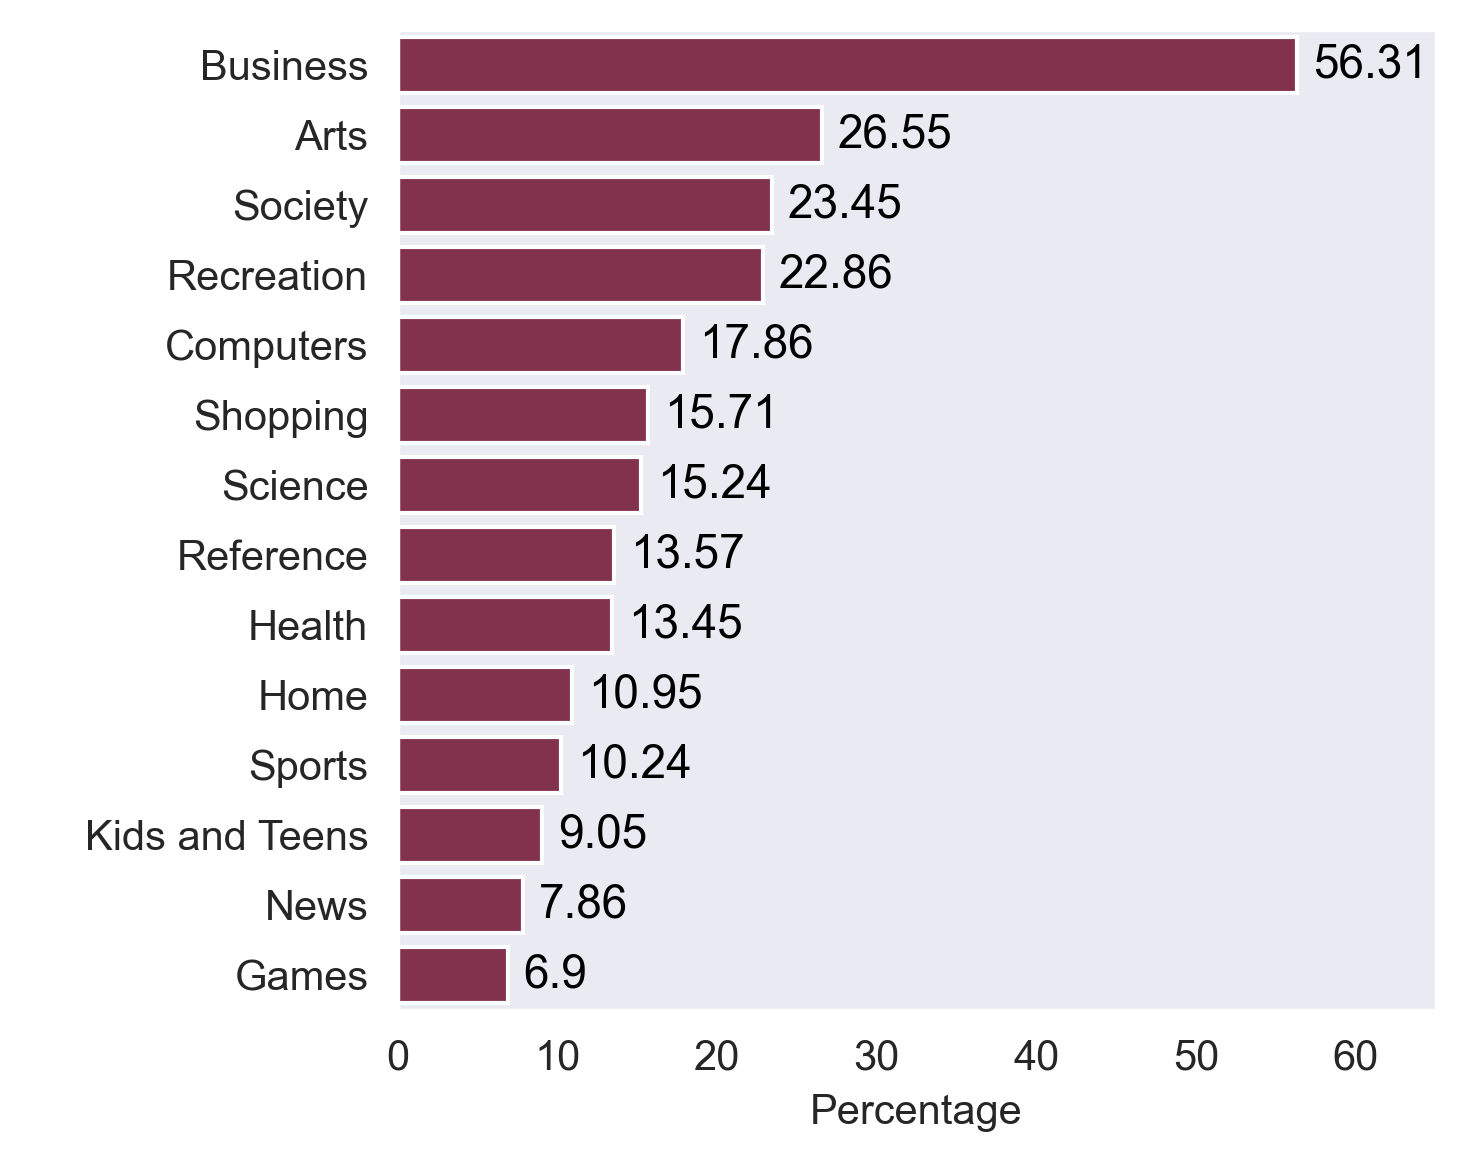
\includegraphics[width=1\columnwidth]{figures/category_distribution.png}
    \caption{Class distribution of the original dataset.}
    \label{fig:class_distribution}
\end{figure}

Figure \ref{fig:class_distribution} illustrates the class distribution of the original dataset. It is imbalanced, with most websites falling into the \textit{Business} category, followed by \textit{Arts} and \textit{Society}. This imbalance, identified in Homepage2vec, negatively impacted model performance on minority classes. We will address this issue in our Methods section.
\section{Methodology}\label{sec:methods}

% Mention the overall goal of our work to keep the big picture in mind
The overall goal of our work is to improve mutlilabel classification performance of the original homepage2vec model \cite{homepage2vec}. 
We refer to this model as \texttt{baseline}. 
We can divide our work into two main phases: (1) obtaining high-quality annotations and (2) fine-tuning the baseline model with the obtained annotations. 
In the following, we describe the methodology for each phase in detail.

\subsection* {Phase 1: Obtaining High-Quality Annotations}
In the first phase, we aim to obtion hight-quality GPT annotations measuring performance against human annotatated data.
The orignal human labaled data comprises of 840 websites, anotated each by 3 diffrent annotators. 
The measured inter-anotator agreement measured by the pairwise Cohen's kappa \cite{cohen-coef} is $0.2 \pm 0.02$, indicating low agreement. 
We assign a category label if at least 2 annotators agree, resulting in an average of $2.5$ labels per website.

For 761 websites that were reachable at the time of writing we scraped their content, extracting features such as top-level domain, domain, title, description, keywords, first 50 links, and first 100 sentences, the same features used in the original Homepage2vec model \cite{homepage2vec} and we used the same pipiline for feature embedding.
Also not all features were available for all websites, as shown in Table \ref{tab:feature_information}.
\begin{table}[!ht]
\centering
\caption{Percentage of websites with each feature accross our datasets.}
\label{tab:feature_information}
\begin{tabular}{lrr}
\toprule
 & Original & Curlie-gpt-10k \\
\midrule
n & 761.00 & 9190.00 \\
tld (\%) & 100.00 & 100.00 \\
domain (\%) & 100.00 & 100.00 \\
tags (\%) & 93.69 & 95.47 \\
titles (\%) & 98.42 & 98.28 \\
descriptions (\%) & 54.93 & 62.95 \\
keywords (\%) & 19.58 & 27.29 \\
links (\%) & 89.88 & 91.62 \\
sentences (\%) & 99.08 & 99.03 \\
\bottomrule
\end{tabular}
\end{table}


This scraped pre-prcessed data is then used to obtain the annotaions using Open-AI API.
The system prompt tells the model to perform a mutlilabel classification (the full prompr can be found in the Appendix \ref{app:prompt}) and to respod in a JSON format with key value pairs representing the category and the binary classification. Additionaly one example can website with the correct label is provided to the model, making it a texttt{1-shot} classificaion.
In the user promept we provided a JSON of the exctrated features, we considered 3 different contexts given to the model, accrding to features important found in the original paper \cite{homepage2vec}. 
The smallest context \texttt{context1} includes the least amount of information about the website, making the classification faster and cheaper as less tokens are used and the \texttt{context3} having all the information about the website that was scraped.

We also considered two versions of the GPT model an older GPT-3.5 model and a newer GPT-4 model, where the GPT-4 model is more expensive and slower to use.
All variants of the Labelers can be found in Tabel \ref{tab:labelers_setup}
% - introduce labelers (parameter dimensions), introduce prompt, one shot example:
\begin{table}[htbp]
    \centering
    \begin{tabular}{lll}
        \toprule
        \textbf{Parameter} & \textbf{Variants} & \textbf{Description} \\
        \midrule
        \texttt{context} 
            & \texttt{context1} & Uses the \texttt{tld}, \texttt{domain}, and \texttt{metatags} \\
            
            & \texttt{context2} & Same as \texttt{context1} plus \texttt{title}, \\ & & \texttt{description} and \texttt{keywords} \\
            
            & \texttt{context3} & Same as \texttt{context2} plus \texttt{links} and \\ & & \texttt{text}\\

        \addlinespace
        \texttt{model} 
            & \texttt{gpt3.5} & Uses GPT-3.5 (\texttt{gpt-3.5-turbo-1106}) \\
            
            & \texttt{gpt4}   & Uses GPT-4 (\texttt{gpt-4-1106-preview}) \\
        
        \addlinespace
        \texttt{fewshot} 
            & \texttt{fewshot} & Injects an example website and label into \\ & & the system prompt \\
            
            & \texttt{zeroshot} & Does not inject any example website or \\ & & label into  the system prompt \\
        \bottomrule
    \end{tabular}
    \caption{Description of Parameters and Variants}
    \label{tab:parameters}
\end{table}

\textbf{Curlie-10k} 
We employ the best-performing GPT annotator evaluated against the human annotated original crowdsourced data to annotate \texttt{curlie-10k}, a dataset with 10k randomly selected websites from Curlie. 
Following the same preprocessing and feature extraction as the original dataset, Table \ref{tab:feature_information} displays feature percentages across datasets. 
As the figure clearly indicates, the most useful features according to the homepage2vec \cite{homepage2vec} descriptions and keywords are missing in around 55 \% and 75 \% of cases, respectively. 

\begin{figure}[!ht]
    \centering
    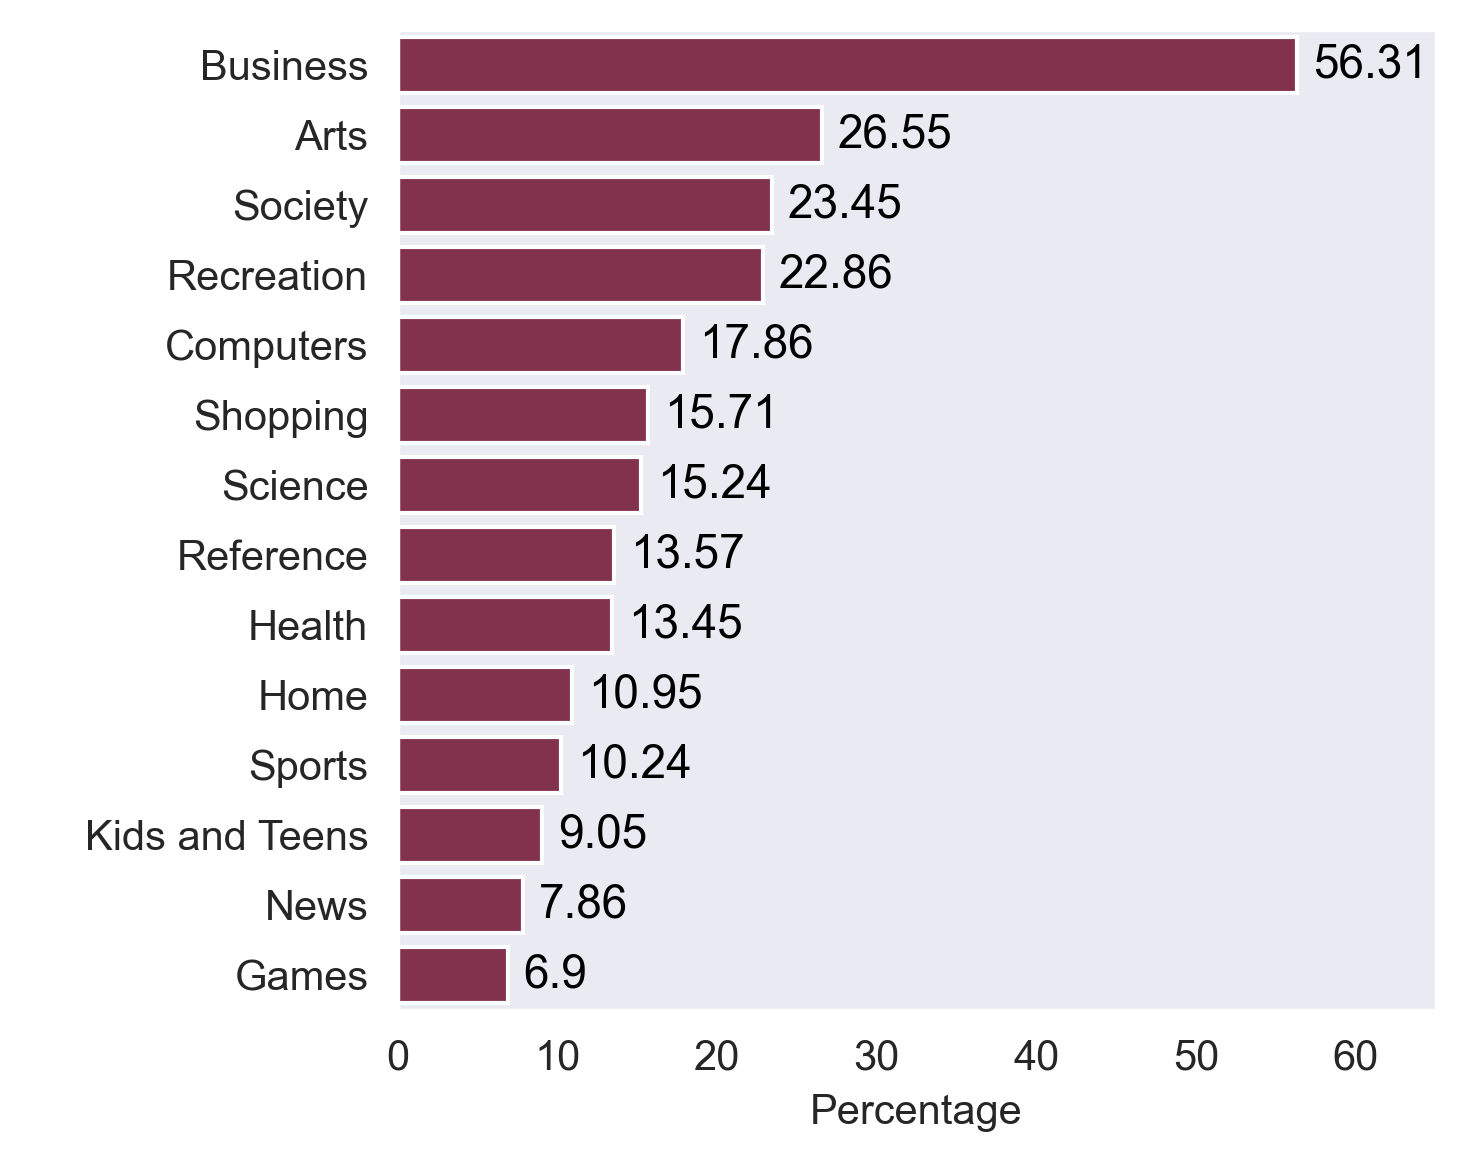
\includegraphics[width=1\columnwidth]{figures/category_distribution.png}
    \caption{Class distribution of the original dataset.}
    \label{fig:class_distribution}
\end{figure}

Figure \ref{fig:class_distribution} illustrates the class distribution of the original dataset. It is imbalanced, with most websites falling into the \textit{Business} category, followed by \textit{Arts} and \textit{Society}. This imbalance, identified in Homepage2vec, negatively impacted model performance on minority classes.
% 1. Step: Show that we can create high-quality annotations (measured against human annotations)
% - introduce curlie (talk about features (missing values), embedding, label list_ , re-scrape + process + embeddin
% ---> All this is pretty much in data, so transfer it here


% 2. Step: Show that we can improve performance compared to pre-trained model via fine-tuning with GPT annotations
% - training parameters (hparams, train/ test data splits)
% - evaluation procedure (macro f1, …)
% - calibration (?)
% TODO: this
\subsection* {Phase 2: Fine-Tuning the Baseline Model}
In the second phase, we fine-tune the baseline model with the obtained annotations from the \texttt{curlie-10k} dataset. And using the crowdsourced data as the test and validation set with 0.7/0.3 split.
We also perform a hyperparmeter search to find the best hyperparameters for the fine-tuning process. 
For this we employ Baeysian TPE samplerer from Optuna \cite{optuna} to efectively search the hyperparam space. 
The hyperparam values are detailed in Table \ref{tab:hyperparameters}.
\begin{table}[!ht]
    \centering
    \caption{\textbf{Hyperparameter Search Space}}
    \label{tab:hyperparameters}
    \begin{tabular}{ll}
    \toprule
    \textbf{Hyperparameter} & \textbf{Search Space} \\
    \midrule
    Learning Rate (\( \lambda \)) & $[0.00001, 0.01]$ \\
    Weight Decay (\( \beta \)) & $[0, 0.1]$ \\
    Scheduler Factor (\(\gamma\)) & $[0.1, 0.5]$ \\
    Batch Size (\(\delta\)) & \{64, 128, 256\} \\
    \bottomrule
    \end{tabular}
\end{table}


The best performing model is chosen by performance on the validation set using the multi-label macro F1 score, which is the average of the F1 score of each class. 
This model is then evaluated on the held out test set using macro F1, precision, recall, and accuracy.




\newpage
\bibliographystyle{IEEEtran}
\bibliography{literature}

\end{document}


% Some important notes from the homepage2vec paper
% 1) Intro
% Before homepage2vec
% - No multilingual models
% - No embeddings based methods
% - Usually paid services
% With Homepage2vec
% - multilingual -> great because out of top 10M websites, 40% are not in English
% - embeddings based
% - open source
% - fast since you can run it locally, and do not have to use external API

% 2) Related work
% Related approaches
% - manual approaches back in the days
% - ML based methods that use contextual features of the given webpage
% - Methods that also use for context the surrounding webpages, especially useful when the current page does not include that much info
% - Methods that use vision features
% - Recently, use of the LSTM, BERT, GRU architectures -> shown to increase performance -> however focus purely on English

% Multilingual embeddings
% - They are using XML-R, multi-lingual model, that has shown to be comparable to the monolingual models

% 3) Dataset
% - Curlie = community edited web directory -> 3M websites in 92 languages,
% labeled in hierarchical categories, however they only used the top level categories
% Originally, there were 15 top level categories, but they dropped "Regional"
% - Majority of classes associated with Bussiness (27), Society (13.9) or Arts (9)
% - 40% of the websites are in English, 16 % in German, 5% in french, 6% in Japanese
% - Although each page may, in principle, have an arbitrary number of category labels, 
% at the top level, the data is mostly single-labeled, with only 2.1% of samples appearing 
% in two or more taxonomy trees of the 14 top-level classes.

% 4) Method
% - They embeded only the first 100 sentences since the embedding process is quite expensive
% This was selected based on the validation set performance using the elbow method
% - They use 19 most frequent domains exluding the domains that indicate country
% - Title, description and keywords are used as well and should be very informative
% - With the links, they use the anchor text and the 50 most frequent texts are used, again
% this was selected using the elbow method